\documentclass{article}
\usepackage[T1,T2A]{fontenc}
\usepackage[utf8]{inputenc}
\usepackage[english,russian]{babel}

\usepackage[left=3cm,right=3cm,
    top=3cm,bottom=3cm,bindingoffset=0cm]{geometry}

\usepackage{graphicx}
\usepackage{color}
\usepackage{hyperref}
\usepackage{amsfonts}
\usepackage{amsmath}

\usepackage{setspace}
\usepackage{indentfirst}
\usepackage{textcomp}
\usepackage{ifthen}
\usepackage{calc}

\title{Теория Вероятностей и Математическая Статистика\\
ФИИТ, 2 курс, 4 семестр}
\author{Лекция 5}

\begin{document}
\maketitle

%\begin{center}
%    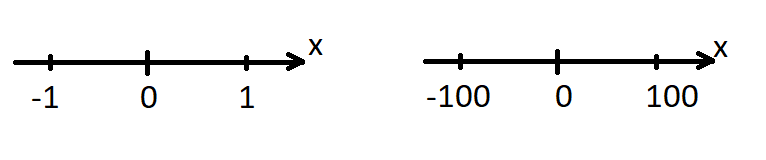
\includegraphics[scale=0.6]{9.png}
%\end{center}

\section{Характеристики распределения случайной величины}

На этой лекции мы продолжим рассмотрение характеристик распределения случайной величины.

\subsection{Квантиль распределения}

Начнем мы с непрерывной случайной величины (НСВ). Для неё квантиль определяется следующим образом:

\textbf{Определение.} Число $x_p$ -- это квантиль распределения $F(x)$ представляет собой решение уравнения:

$$F(x_p) = p,$$

и называется \textbf{квантиль уровня $p$} $(0 < p < 1)$.
\\

\begin{center}
    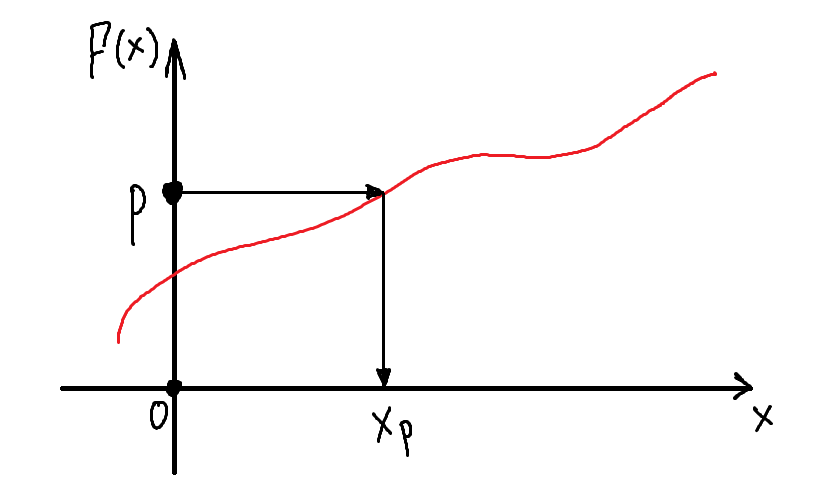
\includegraphics[scale=0.4]{1.png}
\end{center}

\textbf{Замечание 1.} В случае дискретной случайной величины (ДСВ) квантиль определяется в зависимости от задачи.

\textbf{Замечание 2.} В электронном учебнике квантиль относится к \S 5, 6, 7, там же посмотреть определение квантиля в теоретической части учебника, чтобы не сделать ошибку для задач с ДСВ.
 
\subsubsection{Квартиль}

Еще одно понятие, связанное скорее с мат. статистикой. 

\textbf{Квартиль} -- это частный случай квантиля, рассматриваемого для величин $p = 0.25, 0.5, 0.75$.

$p = 0.25, 0.75$ -- нижний и верхний квартили.

$p = 0.5$ -- медиана распределения

\subsubsection{Пример}

Сравним данные за два года, идущих друг за другом. В первом и во втором году были посчитаны средние зарплаты. Причем оказалось, во втором году средняя зарплата стала выше, чем в предыдущем году. При этом будем считать, что инфляция при этом отсутствует. Можно ли сказать, что благосостояние/уровень жизни людей выросло?
\\

Можно рассмотреть много случаев, одни из них:

\begin{enumerate}
\item У людей с низкой зарплатой зарплата стала еще ниже, а у людей с высокой зарплатой наоборот выросла. Разрыв в зарплатах стал наоборот больше, хотя средняя могла повыситься/остаться той же.

\item У всех выросла зарплата, а значит и благосостояние.
\end{enumerate}

Для нас этот вопрос важен с позиции числовых характеристик случайной величины. В общем случае, говорить об однозначном увеличении уровня жизни не приходится. То есть средняя величина, конечно, характеризует что-то, но для полного описания ситуации ее не хватит.

\subsubsection{Пример}

Если рассматривать пример с зарплатами в той же Москве, то мы сможем отметить, что средняя зарплата -- 80к. Но кроме средней зарплаты, есть еще две характеристики:

\begin{enumerate}
\item \textbf{Медианная} -- 50к (47к) -- показывает центральную зарплату. То есть ровно половина населения получает меньше этой суммы, и ровно половина больше. 

\item А так же \textbf{модальная} -- 30к (33к) -- попросту самая распространенная. 
\end{enumerate}

Попробуем показать эти величины на графике плотности какой-нибудь СВ:

\begin{center}
    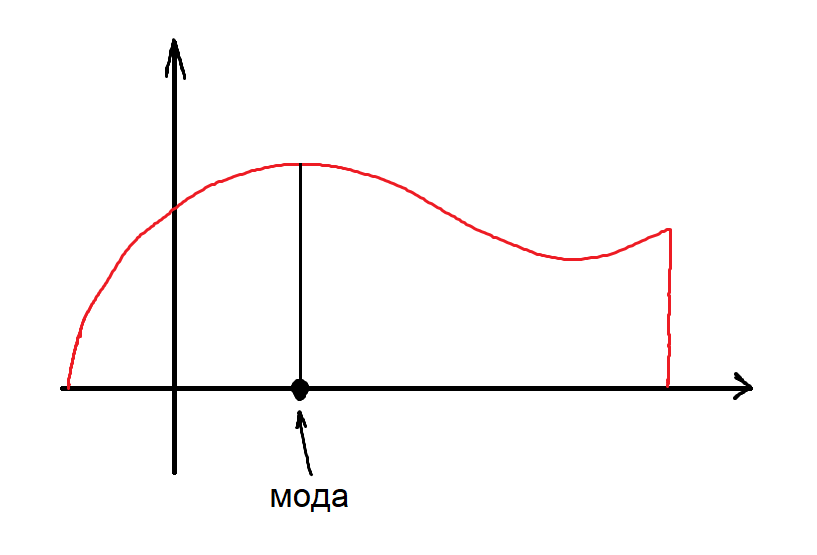
\includegraphics[scale=0.33]{2.png}
    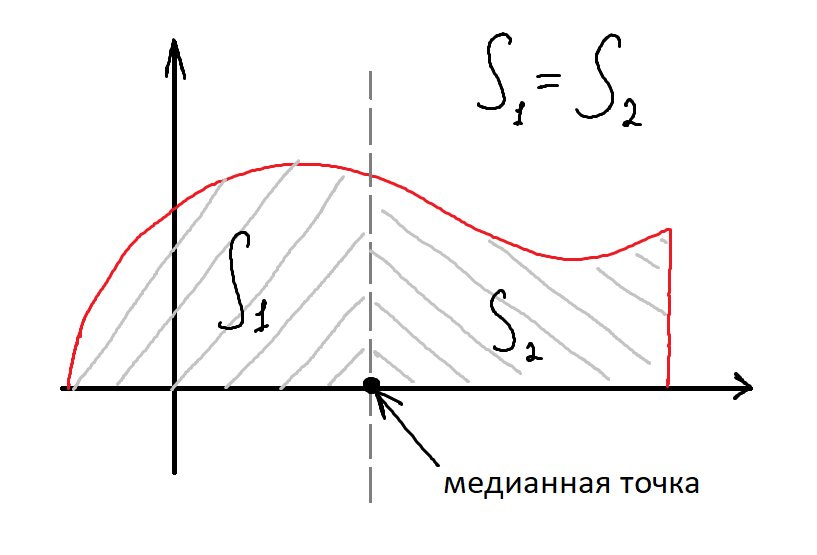
\includegraphics[scale=0.33]{3.png}
\end{center}

\textbf{Модальная} точка (мода) соответствует максимальному значению плотности.

\textbf{Медианная} точка соответствует линии, делящей площадь под графиком пополам.

\textbf{Средняя} точка в данном случае будет считаться как координаты центра тяжести фигуры, как в механике. На этом примерочном графике ее рассчитать достаточно трудно, но нам и так понятно, что значит среднее значение.

\section{Дискретные случайные величины (ДСВ)}

Напомним, что ДСВ характеризует кусочно-постоянная функция распределения, и ее можно задать рядом распределения:

\begin{quote}
$\xi \sim
\begin{pmatrix}
x_1 & x_2 & \ldots & x_n & \ldots\\
p_0 & p_1 & \ldots & p_n & \ldots
\end{pmatrix}$
\end{quote}


То есть перечислить точки разрыва функции распределения и величины скачков в этих точках --- вероятности, отнесенных к этих числовым значениям. Условие нормировки для такой величины --- сходимость ряда: $\sum\limits_{i = 1}^\infty p_i = 1$.

Также напомним себе и о числовых характеристиках ДСВ:

\begin{itemize}
\item \textbf{Математическое ожидание} --- сводится к сумме ряда (если ряд абсолютно сходящийся -- иначе говорят, что величина не имеет мат. ожидания):

$$M\xi = \int\limits_\mathbb{R} xdF(x) =
\sum\limits_{i = 1}^\infty x_i p_i$$

\item \textbf{Дисперсия} --- \textit{второй центральный момент} (гугл):

$$D\xi = \int\limits_\mathbb{R} (x - M\xi)^2 dF(x) =
\sum\limits_{i = 1}^\infty(x - M\xi)^2 p_i$$

Тут же можно отметить мат. ожидание квадрата СВ -- \textit{второй начальный момент} СВ:

$$M\xi^2 = \int\limits_\mathbb{R}x^2dF(x) = \sum\limits_{i = 1}^\infty x_i^2p_i$$

И тогда \textbf{дисперсию} мы можем выразить как разность между \textit{вторым начальным моментом} и \textit{квадратом первого момента}:

$$D\xi = M\xi^2 - (M\xi)^2 = \sum\limits_{i = 1}^{\infty} \xi_i^2 p_i -
\Biggl(\sum\limits_{i = 1}^{\infty} x_i p_i\Biggr)^2$$
\\
\end{itemize}

\subsection{Целочисленные случайные величины}

Вполне понятно, что во всем этом многообразии ДСВ мы захотим выделить некоторую группу наиболее частых -- это \textbf{целочисленные СВ}.
\\

Для работы с этими целочисленными СВ мы введем дополнительную характеристику -- \textbf{производящая функция неотрицательной целочисленной СВ}.

\subsubsection{Производящая функция неотрицательной целочисленной случайной величины}

Пусть наша случайная величина принимает значения с разрывами в целочисленных точках:

\begin{quote}
$\xi \sim
\begin{pmatrix}
0 & 1 & 5 & \ldots & x_n & \ldots\\
p_0 & p_1 & p_2 & \ldots & p_n & \ldots
\end{pmatrix}$
\end{quote}

Обозначим функцию как $\quad\psi(z) = Mz^\xi, \quad$ где $
\begin{cases}
z  \text{-- комплексная переменная}\\
|z| \leq 1
\end{cases}$
\\

Условие $|z| \leq 1$ также можно понимать как "значения $z$ берутся в круге радиуса 1".
\\

Чтобы понять, что нам дает подобная функция, \textbf{найдем ее производную} (в записи штрихи ставить не будем, так как мы ее еще в степень будем возводить, так что будем писать нижний индекс, мол, дифференцируем по $z$: $\psi_z(z)$).

Как мы уже выяснили, мат. ожидание представляет собой интеграл, значит когда мы выполняем действие по дифференцированию у нас возникают две линейные операции: \textit{вычисление производной} и \textit{вычисление интеграла}. Понятно, что их можно менять местами:
 
$$\psi_z(z) = \frac{d}{dz}(Mz^\xi) = M(\frac{d}{dz}z^\xi)$$

Тогда мы можем вполне получить запись такого вида:

$$\psi_z(z) = M(\xi\cdot z^{\xi - 1})$$

При этом значение нашей функции в точке $1$ в точности дает мат. ожидание: $\boxed{\psi_z(1) = M\xi}$.
\\

Ну а теперь, продолжая исследование функции, \textbf{найдем вторую производную} функции. Тогда нам нужно найти производную от выражения, которое стоит внутри мат. ожидания, по той же самой причине, что обе операции линейны:

$$\psi_{zz}(z) = M(\xi(\xi - 1)z^{\xi - 2})$$

И опять же, посмотрим на значение производной в точке $1$:
$$\psi_{zz}(1) = M(\xi^2 - \xi) = M\xi^2 - M\xi$$

Отсюда мы можем выразить \textit{математическое ожидание квадрата}:
$$M\xi^2 = \psi_{zz}(1) + \psi_z(1)$$

И далее наконец можем найти \textit{дисперсию}:
$$\boxed{D\xi} = M\xi^2 - (M\xi)^2 = \boxed{\psi_{zz}(1) + \psi_z(1) - \psi_z^2(1)}$$

\subsubsection{Виды неотрицательных целочисленных случайных величин}

\begin{enumerate}
\item \textbf{Равновероятное распределение.}

Величина принимает конечное количество значений, и каждое значение имеет равную вероятность:

\begin{quote}
$\xi \sim
\begin{pmatrix}
1 & 2 & 3 & \ldots & x_n\\
\frac{1}{n} & \frac{1}{n} & \frac{1}{n} & \ldots & \frac{1}{n}
\end{pmatrix}$
\end{quote}

\textbf{Математическое ожидание} можно расписать следующим образом:

$$M\xi = 1 \cdot \frac{1}{n} + 2 \cdot \frac{1}{n} + \ldots + n \cdot \frac{1}{n} =
\frac{1}{n} (1 + 2 + \ldots + n) = \frac{1}{n} \cdot \frac{n + 1}{2} \cdot n $$

Итого получаем следующую формулу для мат. ожидания:

$$\boxed{
M\xi = \frac{n + 1}{2}
}$$
\\

\textbf{Математическое ожидание квадрата} -- распишем тем же образом, пользуясь формулой для суммы квадратов:

$$M\xi^2 = 1^2 \cdot \frac{1}{n} + \ldots + n^2 \cdot \frac{1}{n} =
\frac{1}{n} \cdot (1^2 + \ldots + n^2) =
\frac{1}{n} \cdot \frac{n(n + 1)(2n + 1)}{6} = \frac{(n + 1)(2n + 1)}{6}$$
\\

\textbf{Дисперсия} (расчеты можно сделать самостоятельно):

$$\boxed{D\xi} = M\xi^2 - (M\xi)^2 = \boxed{\frac{n^2 - 1}{12}}$$ 
\\

\textbf{\textit{Замечание: }} отметим ситуацию, когда величина принимает не обязательно целочисленные значения. но они все еще равновероятные:

\begin{quote}
$\xi \sim
\begin{pmatrix}
x_1 & x_2 & x_3 & \ldots & x_n & \ldots\\
\frac{1}{n} & \frac{1}{n} & \frac{1}{n} & \ldots & \frac{1}{n} & \ldots
\end{pmatrix},$
\end{quote}

\textbf{математическое ожидание} тогда представляет собой среднее арифметическое $\overline{x}$:

$$M\xi = \frac{1}{n} x_1 + \ldots + \frac{1}{n}x_n = \frac{x_1 + \ldots + x_n}{n} = \overline{x}$$
\\
\\

\item \textbf{Распределение Бернулли.}

\textit{(Это распределение, и все остальные виды СВ, будет использовать схему Бернулли.)}

В данном случае, распределение описывает схему Бернулли, состоящую из одного единственного опыта: $n = 1$. То есть опыт оканчивается либо "успехом", либо "неудачей". Таким образом случайную величину можем описать следующим образом:

\begin{quote}
$\xi \sim
\begin{pmatrix}
0 & 1\\
q = 1 - p & p
\end{pmatrix}$
\end{quote}
 
Тогда наши характеристики можно расписать следующим образом:

$$\boxed{M\xi} = 0 \cdot q + 1 \cdot p = \boxed{ p}$$

$$\boxed{D\xi} = p \cdot q = \boxed{ p(1 - p)}$$
\\

\item \textbf{Биномиальное распределение.}

Теперь мы рассматриваем схему Бернулли, в которой проведено $n$ опытов (все еще конечное количество!). Тогда случайную величину можно описать как количество успехов:

\begin{quote}
$\xi \sim
\begin{pmatrix}
0 & 1 & 2 & \ldots & x_n\\
p_0 & p_1 & p_2 & \ldots & p_n
\end{pmatrix}$
\end{quote}

Вероятность соответствующему значению определяется из формулы:

$$p_k = C_n^k \cdot p^k \cdot q^{n - k}$$

Однако теперь вопрос о вычислении \textbf{математического ожидания} становится более существенным,
чем в предыдущих случаях. Попробуем подойти к решению с помощью ранее описанной производящей функции:

$$\psi(z) = Mz^\xi = \sum\limits_{k = 0}^n z^k \cdot C_n^k \cdot p^k \cdot q^{n - k} = $$

Сгруппируем выражения с одинаковой степенью и, заметив разложение Бинома Ньютона, получим:

$$= \sum\limits_{k = 0}^n C_n^k \cdot (zp)^k \cdot q^{n - k} = (zp + q)^n$$
\\

Далее нам потребуется найти первую и вторую производные данной функции:

$$\psi_z(z) = n(zp + q)^{n - 1} \cdot p$$

$$\psi_{zz}(z) = n(n - 1)(zp + p)^{n - 2}\cdot p^2$$
\\

С помощью них можем выразить \textbf{математическое ожидание} по раннее выраженной формуле:

$$M\xi = \psi_z(1) = np(zp + q)^{n - 1} = np(p + q)^{n - 1} = np 
\qquad \textit{// p + q = 1}$$

А также \textbf{дисперсию}:

$$D\xi = M\xi^2 - (M\xi)^2 = \psi_{zz}(1) + \psi_z(1) - \psi_z^2(1) =$$ 
$$ = n(n - 1)p^2 + np - (np)^2 = n^2p^2 - np^2 + np - n^2p^2 = np(1 - p) = npq$$
\\

Таким образом:

$$\boxed{M\xi = np} \qquad\qquad\qquad \boxed{D\xi = npq}$$
\\

\textit{\textbf{Замечание.}} Биномиальное распределение воспроизводимо:

$$\xi = \xi_1 + \xi_2 + \ldots + \xi_n,$$

где $\xi$ задает кол-во успехов в биномиальном распределении в схеме Бернулли для $n$ опытов,
а $\xi_i$ задает распределение в $i$ опыте длинной 1, и может быть выражено как распределение Бернулли (п. 2).
\\

Поэтому для биномиального распределения используется обозначение:

$$\boxed{\xi \sim Bi(n; p)},$$

где величины в этой записи называются \textit{параметрами}: $n$ -- кол-во опытов в схеме Бернулли, $p$ -- вероятность однократного успеха.
\\

А величина, имеющая распределение Бернулли, будет обозначена таким образом: $\xi \sim Bi(1; p)$
\\



\textbf{Наиболее вероятное значение (мода).}

Оно определяется величиной $np - q$, есть два варианта:

\begin{enumerate}
\item Величина \textbf{целая}. Тогда получаются два наиболее вероятных значения:

$\qquad \begin{cases}
m_0^{'} = np - q\\
m_0^{''} = np - q + 1
\end{cases}$

\item Величина \textbf{дробная} -- значение единственное:

$\qquad m_0 = [np - q] + 1$, где $[$ $]$ -- целая часть значения.

\end{enumerate}
\end{enumerate}

\subsubsection{Пример}

Из трехзначных чисел наугад выбрано одно. 

Случайная величина $\xi$ -- количество попарно различных цифр в записи этого числа.

Требуется найти математическое ожидание $M\xi$.
\\

У этой задачи есть два подхода:

\begin{itemize}
\item Первый подход (напрямую).

У нас трехзначное число, тогда сколько попарно различных цифр может быть в записи этого числа? Одна (цифры совпадают), две (две цифры совпадают, но отличаются от третьей) и три (все три различны):

$$\text{3-х значное число}\rightarrow \quad 1,\quad 2,\quad 3 \quad \text{различных цифр}.$$

То есть случайная величина принимает всего 3 значения:

$\xi \sim
\begin{pmatrix}
1 & 2 & 3\\
p_1 & p_2 & p_3
\end{pmatrix}
$

Далее в таком случае можно прорешать и найти мат. ожидание самостоятельно.

\item Второй подход c другой стороны.

Введем не одну, а много случайных величин:

$$\underbrace{\xi_0}_{\text{кол-во нулей}},
\quad \xi_1 \quad,
\quad \ldots \quad ,
\quad \xi_8 \quad , 
\underbrace{\xi_9}_{\text{кол-во девяток}}$$

Тогда наша случайная величина -- это сумма кол-ва нулей, единиц и т.д.:

$$\xi = \underline{\xi_1} + \underbrace{\xi_2 + \ldots + \xi_9}_{\text{рассмотрим сначала их}}$$

Мы рассмотрим сначала кол-во цифр от 1 до 9, по понятным причинам --- число трехзначное и с нуля начинаться не может:

\begin{center}
	$\xi_k \sim
	\begin{pmatrix}
	0 & & 1\\
	& & \\
	\frac{8}{9} \cdot \Bigl(\frac{9}{10}\Bigr)^2 & &
	1 - \frac{8}{9} \cdot \Bigl(\frac{9}{10}\Bigr)^2
	\end{pmatrix}\quad
	k = 1, \ldots, 9\quad$
	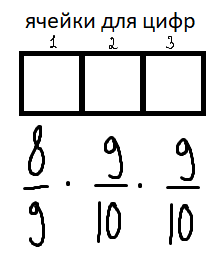
\includegraphics[scale=0.3]{4.png}
\end{center}

И отдельно рассмотрим цифру ноль:
	
$$\xi_0 \sim
\begin{pmatrix}
0 & & 1\\
& & \\
1 \cdot \Bigl(\frac{9}{10}\Bigr)^2 & &
1 - \Bigl(\frac{9}{10}\Bigr)^2
\end{pmatrix}$$

Таким образом, можем найти мат. ожидания:

$$M\xi_0 = 1 - \Bigl(\frac{9}{10}\Bigr)^2;
\qquad M\xi_k = 1 - \frac{8}{9} \cdot \Bigl(\frac{9}{10}\Bigr)^2$$

Осталось только просуммировать мат. ожидания (при расчетах значения $\xi$ для цифр от 1 до 9 одинаковы, поэтому просто умножим одну величину на 9):
 
$$ \xi = \xi_0 + \xi_1 + \ldots + \xi_9$$
$$ M\xi = M\xi_0 + 9 \cdot M\xi_1 + =
1 - \Bigl(\frac{9}{10}\Bigr)^2 + 9 \cdot \Biggl(1 - \frac{8}{9} \cdot \Bigl(\frac{9}{10}\Bigr)^2\Biggr) = 2,71$$
\end{itemize}

\subsection{Геометрическое распределение} 

В этом распределении вновь используется схема Бернулли. Проводится серия опытов, которая рассматривается до наступления первого "успеха". Случайная величина в данном случае -- количество проведенных опытов до наступления "успеха".

$$\xi \sim
\begin{pmatrix}
1 & 2 & 3 & \ldots & x_n & \ldots\\
p_0 & p_1 & p_2 & \ldots & p_n & \ldots
\end{pmatrix}$$

\quad

Как несложно заметить, если случайная величина равна единице, то у нас сразу был успех (возьмем его вероятность за $p$): $\quad P(\xi = 1) = p$.

Если равна двойке, то сначала был неуспех, потом успех: $\quad P(\xi = 2) = q \cdot p$.

$$P(\xi = 3) = q^2 \cdot p \qquad\qquad P(\xi = 4) = q^3 \cdot p$$
$$\boxed{p_n = q^{n - 1} \cdot p}$$

\textit{В качестве задания} --- производящую функцию построить самостоятельно, и с помощью нее найдете мат. ожидание и дисперсию:

$$\boxed{M\xi = \frac{1}{p}} \qquad\qquad \boxed{D\xi = \frac{q}{p^2}}$$

\quad

\textbf{Замечание.} Важно обратить внимание на слово "до [наступления успеха]". Иногда эту случайную величину записывают не включая сам "успех", то есть случайная величина будет начинаться с нуля (ноль "неуспехов" до "успеха"):

$$\xi \sim
\begin{pmatrix}
0 & 1 & 2 & \ldots & x_n & \ldots\\
p_0 & p_1 & p_2 & \ldots & p_n & \ldots
\end{pmatrix}$$

Для такого случая дисперсия не изменится, а мат. ожидание получится со сдвигом на единицу:

$$M\xi = \frac{1}{p} - 1 = \frac{q}{p}$$

\subsubsection{Пример}

Данное распределение можно наблюдать в азартных играх. Случайная величина с таким распределением может дать ответ на вопрос, как наилучшим образом выиграть у казино и вообще, возможно ли это. Построим распределение:

$$\xi \sim
\begin{pmatrix}
1 & 2 & 3 & \ldots \\
p & qp & q^2p & \ldots
\end{pmatrix}$$

Посмотрим на моду этого распределения --- ей будет являться единица ($\xi = 1$).

Буквально, если смотреть на различные вариации достижения <<успеха>> , то <<успех>>  с первой игры более вероятен. Просто потому, что вероятности всех остальных значений гарантированно меньше первого (мы же домножаем на $q, q^2, \ldots$).
\\

То есть если все игроки придут и сыграют один раз и не более (без разницы, <<успех>> ли), таким образом их шансы выиграть будет наивысшим, а если человек будет достаточно много, казино можно вовсе разорить...
\\

Вот такой вот математический взгляд на азартные игры.

\subsubsection{Характеристическое свойство геометрического распределения}

Нам нужно вычислить вероятность:

$$P(\xi = n + k \ |\ \xi > n)$$

В соответствии с формулой условной вероятности, мы получим:

$$ = \frac{P(\xi = n + k,\ \xi > n)}{P(\xi > n)} =
\frac{P(\xi = n + k) }{P(\xi > n)}^\text{// т.к. очевидно, что n + k > n} =$$
$$ = \frac{q^{n + k - 1} p}{q^n p + q^{n + 1}p + \ldots} =
\frac{q^{n + k - 1}p}{q^np)(1 + q + q^2 + \ldots)}_{\text{//бесконечно убывающая прогрессия}} = $$
$$= \frac{q^{n + k - 1}p}{q^np \cdot \frac{1}{1 - q}} = \boxed{q^{k - 1}p}$$

Наше распределение вновь стало геометрическим. Это означает, что если в течение $n$ опытов <<успех>> не наступает, и мы точно знаем о проведении этих опытов, то в целом о них можно просто забыть, и начинать все сначала --- то есть все зависит от дальнейших $k$ опытов.
\\

Можно сказать, что это \textbf{распределение <<не имеет памяти>>}. Это и есть основное \textit{характеристическое свойство} данного распределения.

\end{document}
